\section{Pilot Study}
\label{sec:pilot}

\subsection{Setup}
\label{sec:pilot:setup}

The pilot crosses three LLM families spanning the deployment
spectrum---Claude-Sonnet-4.6 as a frontier closed-weight model,
GPT-5-mini as a mid-tier closed-weight model, and DeepSeek-v4-Flash
as an open-weight reference---with one baseline scenario, three
fixed seeds drawn from a pre-registered list, and two horizons (10
sim-minutes and 60 sim-minutes). The crossing yields eighteen
LLM-driven cells. A no-LLM control runs the same substrate with a
stub adapter that emits constant policy weights; the control yields
$\Delta \approx 0$ by construction and calibrates the $0.3$
hypothesis threshold against substrate noise. Channel cadences are
scaled by a uniform $6\times$ multiplier to fit within an LLM
proxy's per-minute request budget; the multiplier preserves the
relative cadence ratios that produce the dissociation surface.

The pilot is narrower than the design we pre-registered, which
crossed three scenarios, five seeds, and four horizons. The
reduction follows from a sustained rate-limit ceiling on the
proxy we used; broader matrices are the subject of future work
discussed in Section~\ref{sec:limitations}.

\subsection{H1: Existence at Threshold Magnitude}
\label{sec:pilot:h1}

\paragraph{Hypothesis.}
For every LLM family $m$ in the model set, there exists a
sim-time $t \leq 4$\,sim-hours such that $|\Delta(t)| > 0.3$. We
report two horizons (10\,min and 60\,min) and treat the hypothesis
as satisfied when at least one cell per family crosses threshold
or, in aggregate, when the threshold is crossed at all.

\paragraph{Results at 10 sim-minutes.}
All three family means sit in the stale-coherence direction at the
short horizon. Claude-Sonnet-4.6 attains $\bar\Delta = +0.130$,
DeepSeek-v4-Flash $+0.137$, and GPT-5-mini $+0.033$. One of nine
short-horizon cells crosses threshold: a GPT-5-mini seed reaches
$\Delta = +0.380$. The remaining eight cells sit below threshold,
with the family means themselves all in the range $[+0.03, +0.14]$.
At this horizon the dissociation that exists points consistently
toward verbal lead.

\paragraph{Results at 60 sim-minutes.}
The picture changes substantially at the longer horizon. Three of
nine cells cross threshold, and all three sit in the action-lead
direction ($\Delta < 0$): DeepSeek-v4-Flash crosses on two of
three seeds (with $\Delta$ reaching $-0.43$), and GPT-5-mini
crosses on one seed ($\Delta = -0.32$). Combining both horizons,
four of eighteen pilot cells exceed $|\Delta| > 0.3$, of which one
is verbal-lead and three are action-lead. Existence is
established: the dissociation reaches threshold magnitude on the
pilot, and it does so within one sim-hour rather than requiring
the four-hour horizon. Table~\ref{tab:e1-stageb} reports the
per-family aggregate at the 60-minute horizon;
Figure~\ref{fig:alpha:trajectory} overlays the trajectories.

\begin{figure}[t]
  \centering
  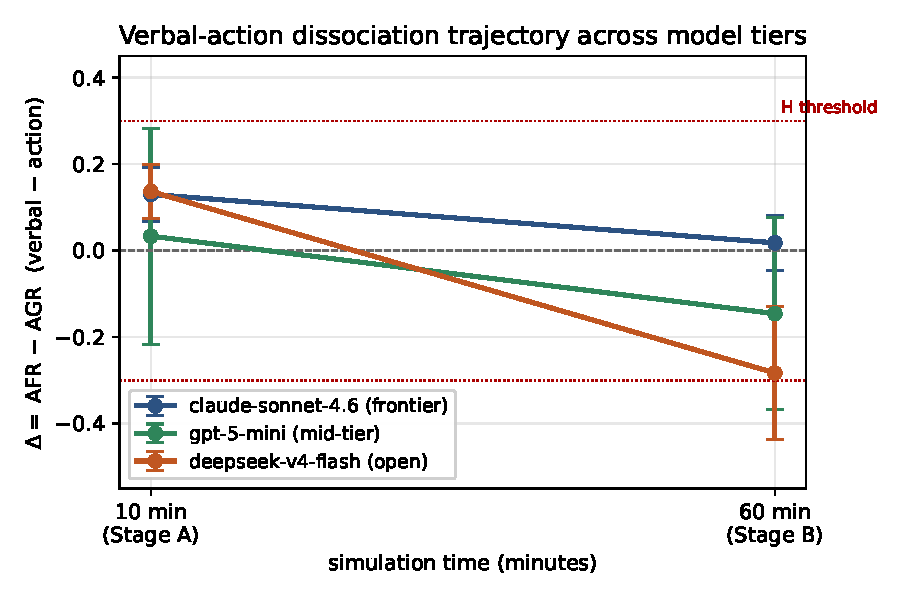
\includegraphics[width=0.95\linewidth]{figures/fig_route_alpha_delta_trajectory.pdf}
  \caption{Per-family mean dissociation gap $\bar\Delta(t)$ at the
  two pilot horizons, with $\pm 1\sigma$ across three seeds. Red
  dotted lines mark the $|\Delta| = 0.3$ threshold. Claude trends
  toward coherence; the two weaker families flip sign and grow in
  magnitude.}
  \label{fig:alpha:trajectory}
\end{figure}

\begin{table}[t]
  \centering
  \scriptsize
  \setlength{\tabcolsep}{3pt}
  \begin{tabular}{l c c r c}
    \toprule
    Model & AFR & AGR & $\bar\Delta$ & thr.\ \\
    \midrule
    Claude-Sonnet-4.6  & $0.82{\pm}0.08$ & $0.80{\pm}0.00$ & $+0.02{\pm}0.08$ & $0/3$ \\
    GPT-5-mini         & $0.37{\pm}0.01$ & $0.52{\pm}0.27$ & $-0.15{\pm}0.27$ & $1/3$ \\
    DeepSeek-v4-Flash  & $0.47{\pm}0.13$ & $0.75{\pm}0.06$ & $-0.28{\pm}0.19$ & $\mathbf{2/3}$ \\
    \bottomrule
  \end{tabular}
  \caption{Per-family dual probe at the 60-minute horizon
  (mean~$\pm$~sample~std, $n = 3$ seeds). The ``thr.'' column
  reports the number of seeds per family whose $|\Delta|$
  exceeds the pre-registered $0.3$ threshold. Families are
  ordered by deployment tier (frontier first).}
  \label{tab:e1-stageb}
\end{table}

\subsection{Observation 1: Tier Stratification}
\label{sec:pilot:tier}

Dissociation magnitude at the 60-minute horizon orders cleanly by
deployment tier. The mean $|\bar\Delta|$ is $0.018$ for
Claude-Sonnet-4.6, $0.146$ for GPT-5-mini, and $0.283$ for
DeepSeek-v4-Flash. The frontier model maintains coherence between
its verbal and action channels; the mid-tier closed model exhibits
a moderate dissociation; the open-weight model approaches the
threshold on its mean and crosses it on two of three seeds.
Figure~\ref{fig:alpha:dual} shows the underlying AFR and AGR
contributions: DeepSeek's verbal recall collapses while its action
grounding stays high, GPT-5-mini exhibits a weaker version of the
same gap, and Claude maintains both.
Figure~\ref{fig:alpha:tier} summarises the tier ordering as a bar
chart against the threshold.

We report this ordering as an observation rather than as a
statistical claim. With three seeds per family the standard
deviation across seeds is comparable in magnitude to the
between-family differences, and the strict ordering should be
interpreted as a pattern to be tested in a broader matrix rather
than as a confirmed tier law.

\begin{figure}[t]
  \centering
  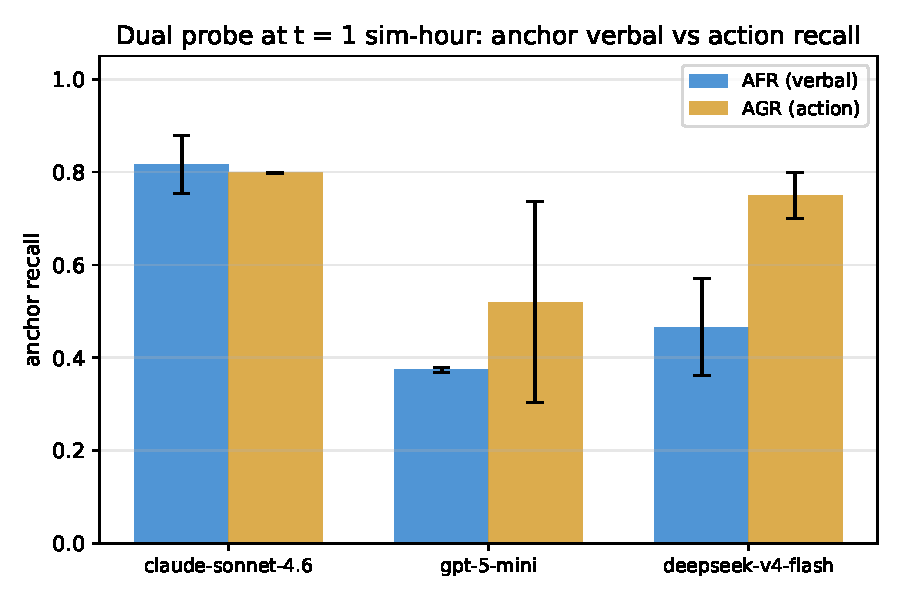
\includegraphics[width=0.95\linewidth]{figures/fig_route_alpha_dual_probe.pdf}
  \caption{Dual probe at the 60-minute horizon: anchored fact
  recall (AFR, blue) and action-grounded recall (AGR, gold) per
  family. DeepSeek's AFR collapses while AGR stays high;
  GPT-5-mini exhibits the same gap with smaller magnitude; Claude
  maintains both. Error bars are $\pm 1\sigma$ across three seeds.}
  \label{fig:alpha:dual}
\end{figure}

\begin{figure}[t]
  \centering
  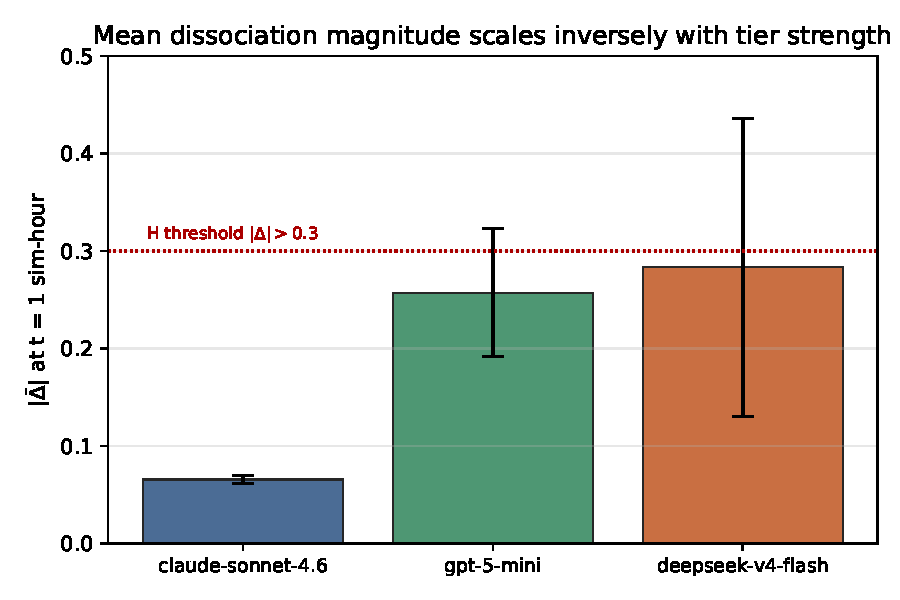
\includegraphics[width=0.85\linewidth]{figures/fig_route_alpha_tier_dissociation.pdf}
  \caption{Mean dissociation magnitude $|\bar\Delta|$ at the
  60-minute horizon by family. The hypothesis threshold (red
  dotted) sits at $0.3$. The frontier model maintains coherence;
  the open-weight model crosses threshold on two of three seeds.}
  \label{fig:alpha:tier}
\end{figure}

\subsection{Observation 2: Horizon-Dependent Direction}
\label{sec:pilot:horizon}

The sign of $\Delta$ depends on the horizon. At 10\,minutes all
three family means are positive ($+0.130$, $+0.137$, $+0.033$). At
60\,minutes DeepSeek and GPT-5-mini flip to negative ($-0.283$ and
$-0.146$ respectively), while Claude attenuates toward zero
($+0.018$). Paired per-seed differences from the short to the long
horizon are $-0.112$ for Claude, $-0.420$ for DeepSeek, and
$-0.179$ for GPT-5-mini. We frame this regularity as a directional
observation: in two of three families the dissociation reverses
sign with horizon, and the frontier model does not. With three
seeds per cell we cannot mount a strong claim about the dynamics
of the reversal; we report the pattern because it is consistent
across the two non-frontier families and because it has direct
implications for deployment, where the direction of dissociation
determines which monitoring signal catches the failure.

\subsection{H2: Independence from Verbal Recall}
\label{sec:pilot:h2}

\paragraph{Hypothesis.}
A pre-registered corollary asked whether $\Delta$ is independent
of a verbal-only recall proxy. The version of this test we
originally reported used AFR itself as the proxy, but AFR is by
construction a component of $\Delta = \mathrm{AFR} - \mathrm{AGR}$,
and when AGR is approximately constant per model
($\mathrm{AGR}\!\approx\!0.80$ for Claude, $0.68$--$0.78$ for
DeepSeek, $0.21$--$0.69$ for GPT-5-mini) the magnitude
$|\Delta|=|\mathrm{AFR}-\mathrm{AGR}|$ is mathematically tied to
AFR. Any correlation $\rho(|\Delta|,\mathrm{AFR})$ therefore has a
mechanical floor that is partly an artefact of AGR's per-model
stability rather than an empirical finding. We replace the
self-referential AFR proxy with an \emph{external} verbal-recall
probe, designed to be definitionally independent of every pilot
quantity.

\paragraph{External probe design.}
The external probe is a standalone LongMemEval-style
needle-in-haystack benchmark, run on the same three models, three
seeds, and two context-length conditions as the pilot. Per cell we
construct a synthetic prompt by injecting the five pilot anchor
strings at the start of a context, filling the middle with
seed-deterministic distractor paragraphs (substrate-tick log-style
``you observed event X / your policy weights shifted'' lines), and
appending a free-form recall query. The synthetic context targets
${\sim}4\,000$ tokens for the 10-min condition and ${\sim}25\,000$
tokens for the 60-min condition, matching the order-of-magnitude
context length the corresponding pilot cell accumulates. Scoring
is per-anchor: $1.0$ for both verbal token and action recalled,
$0.5$ for either half, $0.0$ for neither; the cell score is the
mean across the five anchors. The probe touches no part of the
substrate: it has no AGR, no $\Delta$, no policy directives, no
worker grounding. It is the same retrieval test that
LongMemEval-style benchmarks measure, applied to the same models
at the same orders of context length. Appendix~B in supplementary
material details the prompt template and the deterministic
distractor generator.

\paragraph{Results.}
Sixteen of the eighteen cells produced real-LLM responses on the
external probe; two Claude-Sonnet-4.6 60-min cells failed when the
proxy wallet was exhausted by the ${\sim}25{,}000$-token prompts
and could not be recovered within the study window. Across the
sixteen recovered cells, \emph{every model recalled every anchor
in every cell}: the external recall score is $1.000$ in every
joinable observation. Because the external recall column is
constant, Spearman $\rho(|\Delta|, \mathrm{external\_recall})$ is
mathematically undefined; we therefore report the ceiling outcome
rather than a numerical correlation. Table~\ref{tab:h2-external}
reports the per-condition aggregate.

\begin{table}[t]
  \centering
  \scriptsize
  \setlength{\tabcolsep}{3pt}
  \begin{tabular}{l c r r c c}
    \toprule
    Model & Hzn & $\bar\Delta$ & $|\Delta|$ rng & ext. & $n_{\mathrm{rec}}$ \\
    \midrule
    Claude-Sonnet-4.6  & 10\,m & $+0.13$ & $[.05,.20]$ & $1.00$ & $3/3$ \\
    Claude-Sonnet-4.6  & 60\,m & $+0.02$ & $[.06,.07]$ & $1.00$ & $1/3$ \\
    GPT-5-mini         & 10\,m & $+0.03$ & $[.08,.38]$ & $1.00$ & $3/3$ \\
    GPT-5-mini         & 60\,m & $-0.15$ & $[.17,.32]$ & $1.00$ & $3/3$ \\
    DeepSeek-v4-Flash  & 10\,m & $+0.14$ & $[.07,.22]$ & $1.00$ & $3/3$ \\
    DeepSeek-v4-Flash  & 60\,m & $-0.28$ & $[.07,.43]$ & $1.00$ & $3/3$ \\
    \bottomrule
  \end{tabular}
  \caption{Pilot $\Delta$ joined against the external verbal-recall
  probe, aggregated per (model, horizon) condition ($n = 3$ seeds
  per condition). $\bar\Delta$ averages the substrate $\Delta$
  across the three pilot seeds; $|\Delta|$ range reports the span
  across the same three seeds. The external recall column
  averages over the recovered external-probe runs only;
  $n_{\mathrm{rec}}$ reports how many of three external probes
  completed (two Claude 60-min runs failed due to proxy quota
  exhaustion). External recall is constant at $1.00$ across all
  sixteen recovered cells.}
  \label{tab:h2-external}
\end{table}

\paragraph{Reading.}
The ceiling outcome is a stronger decoupling result than a low
$|\rho|$ would have been. The two pilot cells with the largest
$|\Delta|$---both DeepSeek-v4-Flash at the 60-minute horizon, with
$\Delta = -0.43$ and $-0.35$, exhibiting collapsed pilot AFR in
the $0.36$--$0.43$ range---recall the external anchors perfectly
when asked the same retrieval question outside the substrate loop. The collapsed-AFR signature inside the dual probe
is therefore not the same failure mode that LongMemEval-style
benchmarks measure; if it were, the same models on the same orders
of context length would have failed the external probe too. We
read this as evidence that the dual probe's $\Delta$ measures a
substrate-coupled failure that a single-axis verbal-recall
benchmark would render invisible. Two qualifications remain:
sixteen cells is a narrow matrix to claim full independence, and
the perfect external recall is itself a ceiling effect that a
harder probe might puncture. We therefore frame the result as
\emph{independence supported on the pilot}, leaving room for a
broader matrix and a harder external probe in follow-on work.
